\documentclass[10pt]{beamer}

%\usetheme[bullet=square,titleline=true,alternativetitlepage=true]{Torino}

\usepackage[absolute,overlay]{textpos}

\usepackage{pdflscape}
\usepackage{psfrag} 
\usepackage{epsfig}
\usepackage{thumbpdf}
\usepackage{graphicx,graphics}
\usepackage{multirow,multicol}
\usepackage{amsmath,amssymb}
\usepackage{hyperref}
\usepackage{ulem}
\usepackage{times}
\usepackage{bm}
\usepackage{fancybox}
\usepackage{algorithm,algorithmic}
\usepackage{listings}

\usepackage{multimedia}
\usepackage{media9}
\newcommand{\pdfmovie}[4]{\href{run:#1}{\framebox{\parbox[c][#3][c]{#2}{\center #4}}}}


%\usepackage[T1]{fontenc} 
\usepackage[latin9]{inputenc}

\usepackage{tikz,xcolor,tcolorbox}
\usetikzlibrary{mindmap,trees}

\setcounter{secnumdepth}{2}
\setcounter{tocdepth}{2}

%indicatrice
\def\1{\mbox{1\hspace{-.22em}I}}

\newcommand{\pdf}{\mbox{p}}

\newcommand{\bg}{\bold{g}}
\newcommand{\ba}{\bold{a}}
\newcommand{\bu}{\bold{u}}
\newcommand{\bX}{\bold{X}}
\newcommand{\bY}{\bold{Y}}
\newcommand{\bM}{\bold{M}}
\newcommand{\bV}{\bold{V}}
\newcommand{\bB}{\bold{B}}
\newcommand{\bW}{\bold{W}}
\newcommand{\bZ}{\bold{Z}}


\newcommand{\bx}{\bold{x}}
\newcommand{\be}{\bold{e}}
\newcommand{\by}{\bold{y}}
\newcommand{\bz}{\bold{z}}
\newcommand{\bc}{\bold{c}}
\newcommand{\bt}{\bold{t}}
\newcommand{\bmu}{\boldsymbol{\mu}}
\newcommand{\bpi}{\boldsymbol{\pi}}
\newcommand{\balpha}{\boldsymbol{\alpha}}
\newcommand{\bbeta}{\boldsymbol{\beta}}
\newcommand{\btheta}{\boldsymbol{\theta}}
\newcommand{\bw}{\bold{w}}
\newcommand{\bv}{\bold{v}}


%\let\origdescription\description
%\renewenvironment{description}{
%    \origdescription
%  %  \setlength{\leftmargin}{-300ex}
%    \setlength{\labelsep}{1ex}
%   \setlength{\itemindent}{0ex}
%\setlength{\listparindent}{\parindent}
%}

%\let\origdescription\description
%\renewenvironment{description}{
%  \setlength{\itemsep}{-20ex}
%  \origdescription
%  \setlength{\itemindent}{-1em}
%  \setlength{\labelsep}{\textwidth}
%  \setlength{\listparindent}{\parindent}
%}
%{\endlist}

\def\relief#1{{\color{blue} {#1}}}

\newcommand{\argmax}{\mathop{\mathrm{argmax}}}
\newcommand{\argmin}{\mathop{\mathrm{argmin}}}

\def\1{\mbox{1\hspace{-.22em}I}}

\let\origdescription\description
\renewenvironment{description}{
    \origdescription
    \setlength{\leftmargin}{-30ex}
    \setlength{\itemindent}{-5.25ex}
    \setlength{\labelsep}{1.5ex}
   \setlength{\itemindent}{0ex}
\setlength{\listparindent}{\parindent}
}
{\endlist}


\author[F.-X. JOLLOIS]{Fran\c{c}ois-Xavier JOLLOIS\\ Universit\'e Paris Descartes, France}
\institute[Univ Paris]{\textit{joint work with \\C. Bouveyron (Univ. Nice), L. Bozzi (EDF) \& J. Jacques  (Univ. Lyon)}}

\title[Functional Latent Block Model]{Functional Latent Block Model}
\subtitle{for functional data co-clustering}

\date{}

\AtBeginSubsection[]
{
\begin{frame}<beamer>
  \frametitle{Contents}
  \tableofcontents[currentsection,currentsubsection]
\end{frame}
}

\AtBeginSection[]
{
\begin{frame}<beamer>
  \frametitle{Plan}
  \tableofcontents[currentsection]
\end{frame}
}

%%%%%%%%%%%%%%%%%%%%%%%%%%%%%%%%%%%%%%%%%%%%%%%%%
%%%%%%%%%%%%%%%%%%%%%%%%%%%%%%%%%%%%%%%%%%%%%%%%%
\begin{document}
%%%%%%%%%%%%%%%%%%%%%%%%%%%%%%%%%%%%%%%%%%%%%%%%%
%%%%%%%%%%%%%%%%%%%%%%%%%%%%%%%%%%%%%%%%%%%%%%%%%

\begin{frame}
\titlepage
\end{frame}


\begin{frame}
\frametitle{The data}
\begin{itemize}
\item \relief{electricity consumption} measured by Linky meters for EDF
\item \relief{27 millions} of customers / \relief{730 daily} consumption over 2 years
\begin{figure}
%\begin{center}
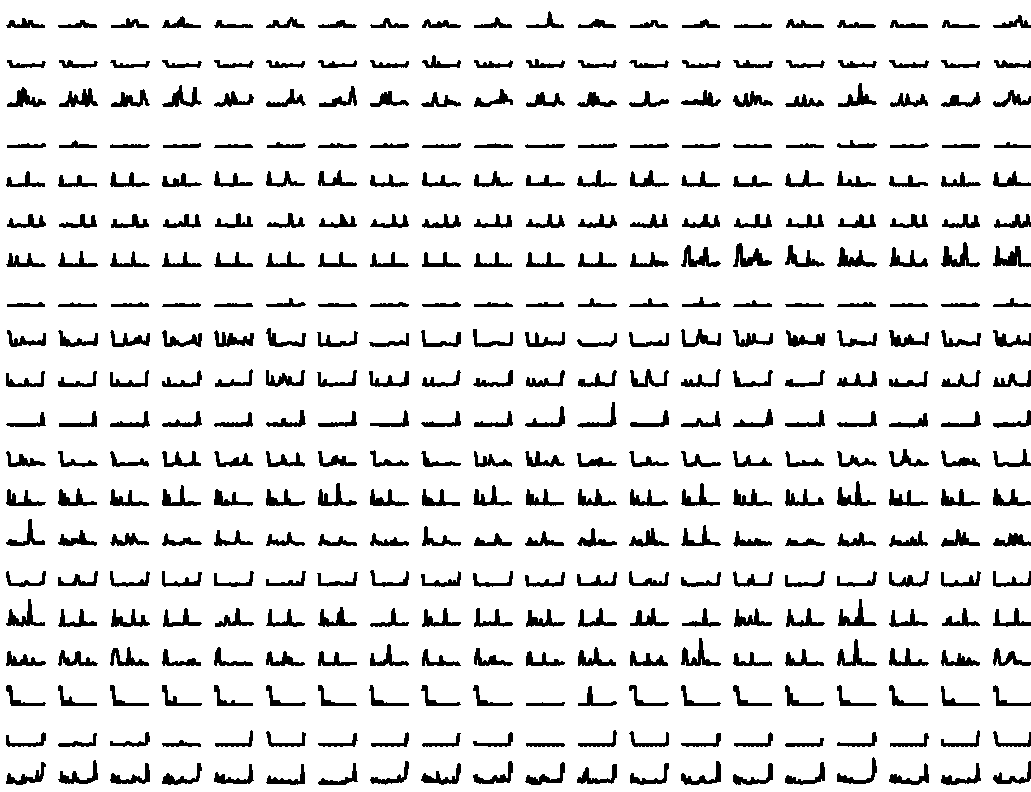
\includegraphics[width=6cm]{images/dataEDF.pdf}
%\end{center}
\caption{Sample of 20 consumptions for 20 days}
\end{figure}
\end{itemize}
\end{frame}

\begin{frame}
\frametitle{The data}
\begin{itemize}
\item large data matrix $\bx=(x_{ij}(t))_{1\leq i \leq n, 1\leq j \leq p}$
\item there is a need to \relief{summarize this data flow}
\item \relief{both} $n$ and $p$ are (very) \relief{large}
\item[$\Rightarrow$] need for \relief{clustering of row} (customers) \alert{and} \relief{column} (days of consumption):
\begin{center}
\alert{need for co-clustering of functional data}
\end{center}
\end{itemize}
\end{frame}


%\begin{frame}
%\frametitle{The data}
%\begin{figure}
%\begin{center}
%\includegraphics[width=5cm]{images/data4.pdf}
%\end{center}
%\end{figure}
%\vspace{-1cm}
%\begin{block}{Our goal}
%\begin{itemize}
%\item to help the support team in identifying \relief{troubleshooting}
%\item to extract a \relief{synthetic summary} of data for the support team by \relief{grouping together}
%\begin{itemize}
%\item similar daily evolutions (row)
%\item similar KPI (column)
%\item \alert{$\Rightarrow$ we need a co-clustering approach for functional data}
%\end{itemize}
%\end{itemize}
%\end{block}
%\end{frame}


\begin{frame}
\frametitle{Co-clustering ?}
Simultaneous clustering of rows (individuals) and column (features)
\begin{figure}[h]
\centerline{
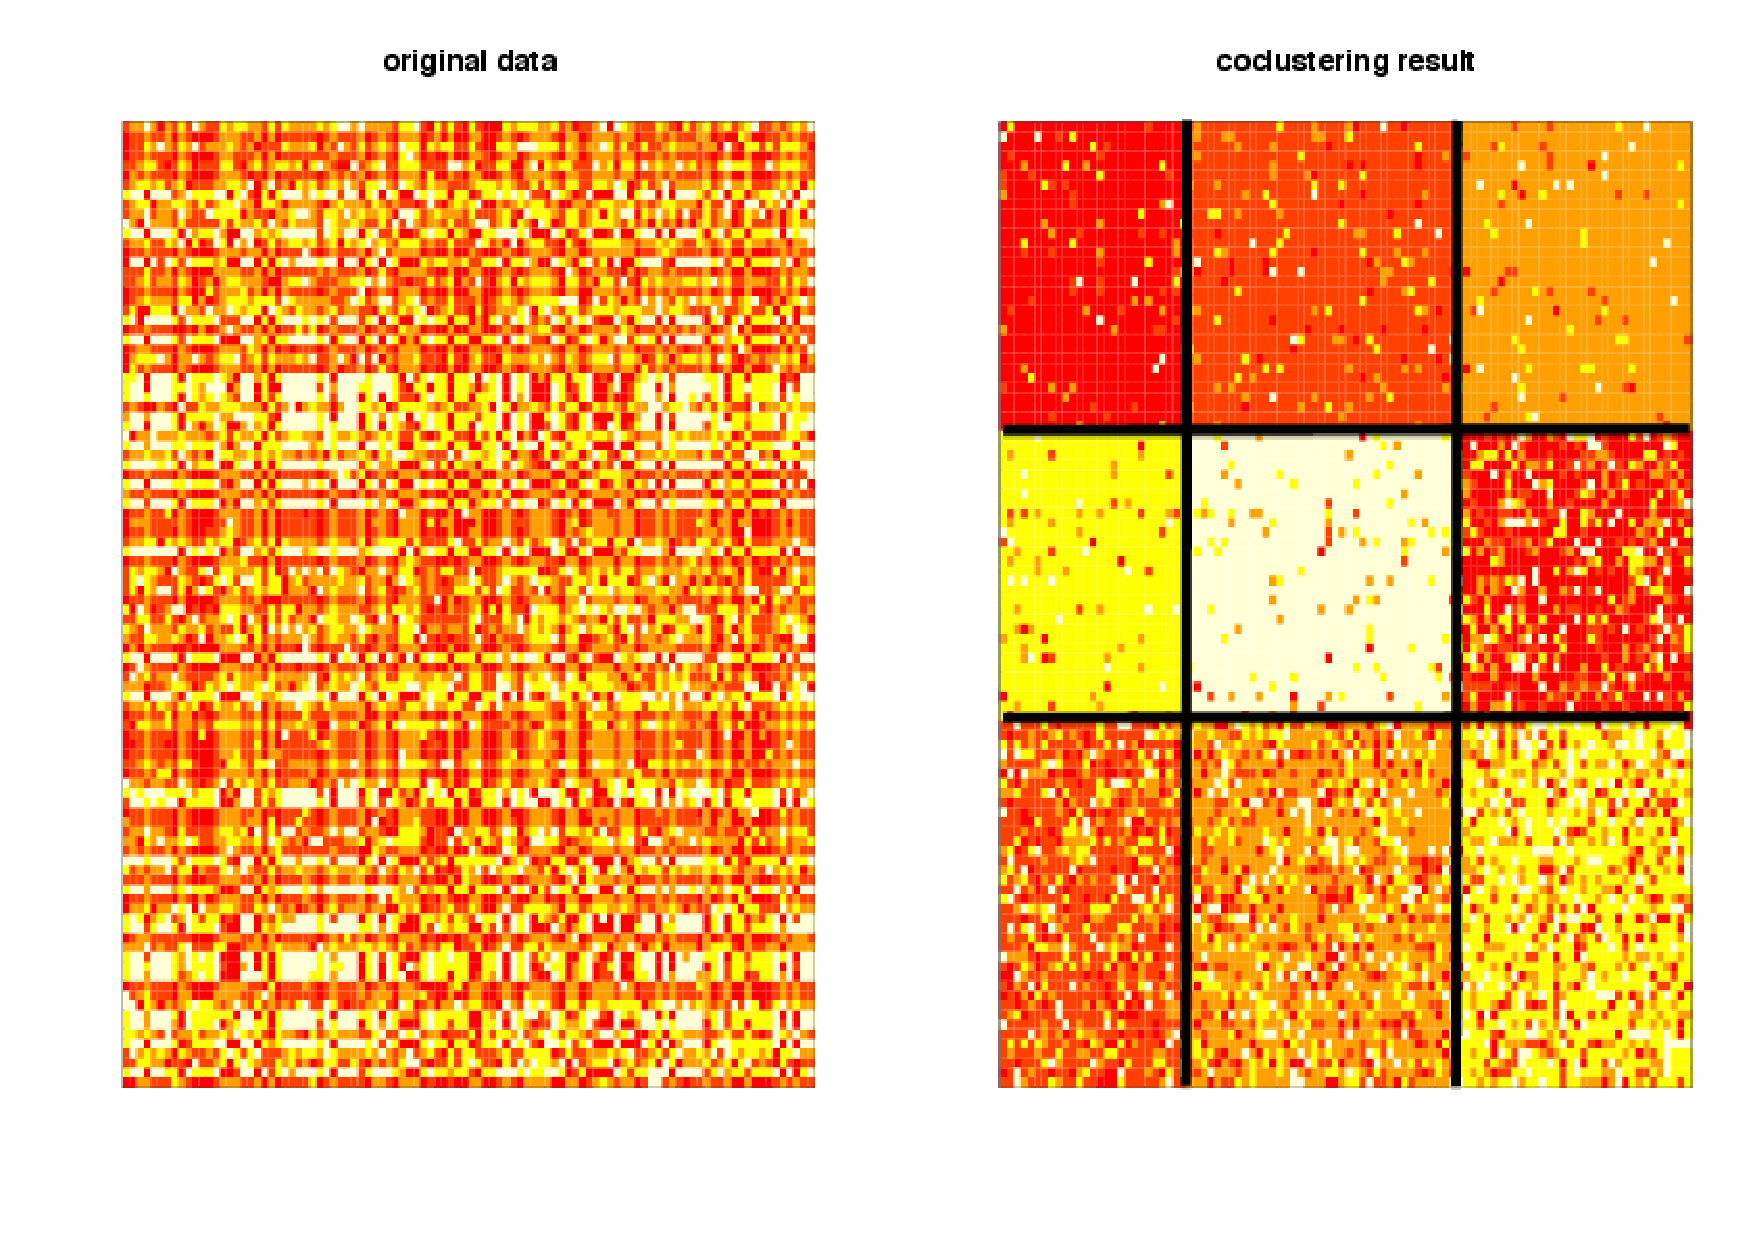
\includegraphics[height=5cm,width=10cm,angle=0]{images/Simul1-data.pdf}
}
\end{figure}
\vspace{-1cm}
legend: color level = $\frac{1}{T}\int_{T}x_{ij}(t)$
\end{frame}

\begin{frame}
\frametitle{Electricity consumption = functional data}
\begin{itemize}
\item $x_{ij}(t)$ are not totally known but only observed at a finite number of times points $x_{ij}(t_1),x_{ij}(t_2),\ldots$
\item need to reconstruct the functional nature of data
\item[$\Rightarrow$] basis expansion assumption: 
\begin{eqnarray*}
x_{ij}(t)=\sum_{h=1}^{m}a_{ijh}\phi_{h}(t), \quad t\in[0,T].
\end{eqnarray*}
where $(\phi_{h}(t))_h$ : spline, Fourier, wavelets...
\item $a_{ijh}$ estimated by least square smoothing
\end{itemize}
\end{frame}

\begin{frame}
\frametitle{Overview} 
\tableofcontents
\end{frame}

\section{The fLBM model}

\begin{frame}{Latent Block Model (LBM)}
\begin{block}{Assumptions}
\begin{itemize}
\item row $\bz=(z_{ik})_{i,k}$ and column $\bw=(w_{h\ell})_{h,\ell}$ partitions are independent
\item conditionally on $(\bz,\bw)$, $x_{ij}$ are independent and generated by a block-specific distribution:
\end{itemize}
\begin{minipage}[c]{.36\linewidth}
\hfill$\pdf{(\theta_{k\ell})}$
   \end{minipage}
   \begin{minipage}[c]{.46\linewidth}
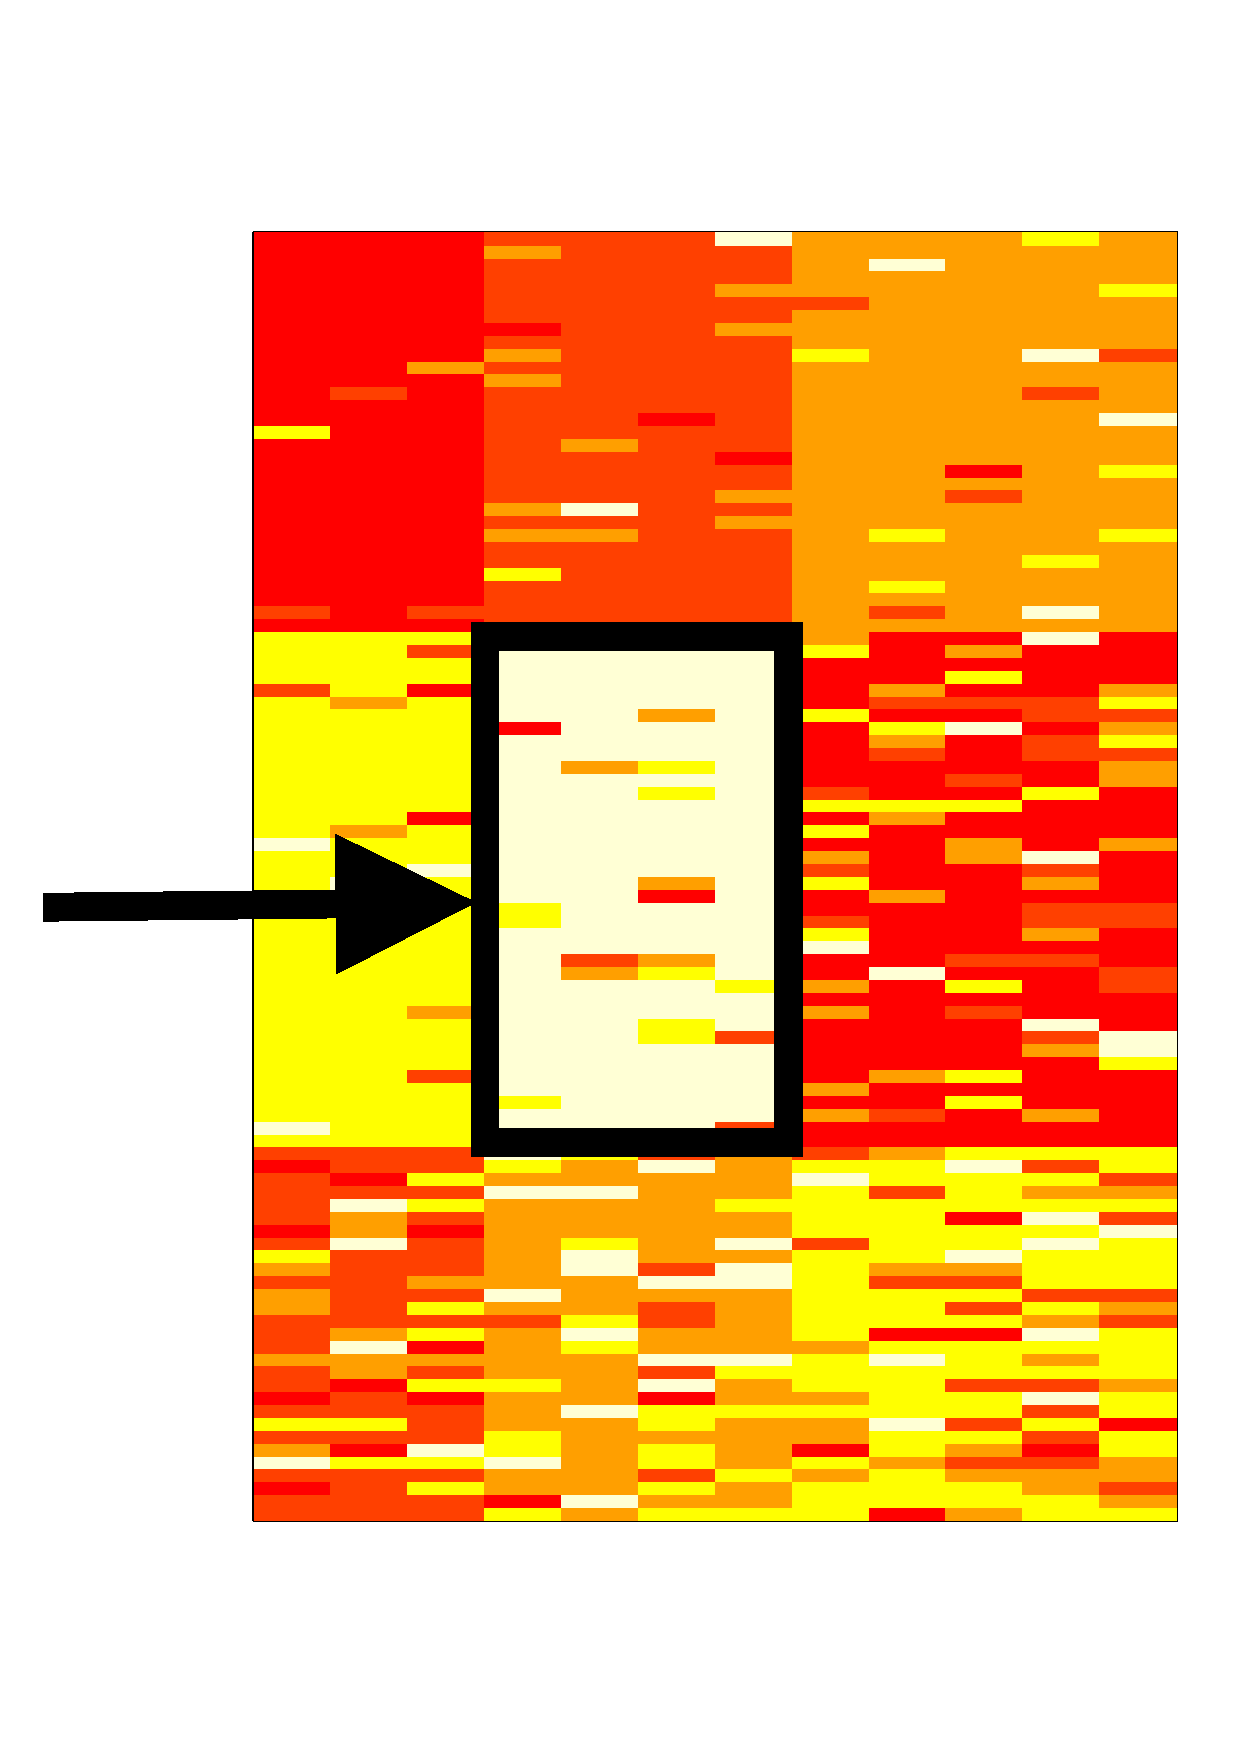
\includegraphics[height=5cm,width=5cm,angle=0]{images/LBM2.pdf}
   \end{minipage}
\end{block}
\end{frame}

\begin{frame}{Latent Block Model}
\begin{block}{Latent Block Model (LBM)}
$n \times d$ random variables $\bx$ are assumed to be independent once the row $\bz=(z_{ik})_{i,k}$ and column $\bw=(w_{h\ell})_{h,\ell}$ partitions are fixed:
\begin{eqnarray*}
\pdf(\bx;\theta) = \sum_{\bz\in V}\sum_{\bw\in W} \pdf(\bz;\theta)\pdf(\bw;\theta)\pdf(\bx|\bz,\bw;\theta)
\end{eqnarray*}
with
\begin{small}
\begin{itemize}
\item $V$ ($W$) set of possible partitions of rows (column) into $K$ ($L$) groups,
\item $\pdf(\bz;\theta)=\prod_{ik}\alpha_k^{z_{ik}}$ and $ \pdf(\bw;\theta)=\prod_{h\ell}\beta_{\ell}^{w_{h\ell}}$
\item $\pdf(\bx|\bz,\bw;\theta)=\prod_{ijk\ell} \pdf(\ba_{ij};\theta_{k\ell})^{v_{ik}w_{h\ell}}$% where
%\begin{itemize}
%\item $\pdf(\cdot;\theta_{k\ell})$ is the block specific distribution
%\end{itemize}
\item $\theta=(\alpha_k,\beta_{\ell},\theta_{k\ell})$
\end{itemize}
\end{small}
\end{block}
\end{frame}

\begin{frame}{The functional Latent Block Model (fLBM)}
\begin{small}$\pdf(\ba_{ij};\theta_{k\ell})$ is the funHDDC distribution \textit{(Bouveyron \& Jacques, ADAC, 2011)}:
$$\ba_{ij}|(z_{ik}=1,w_{j\ell}=1)\sim\mathcal{N}(U_{k\ell}\mu_{k\ell},U_{k\ell}\Sigma_{k\ell}U_{k\ell}^t+\Xi_{k\ell})$$
where
\begin{itemize}
\item $U_{k\ell}$ projects the $\ba_{ij}$ into a low dimensional subspace for block $k\ell$
%defines such that the orthogonal $m \times m$ matrix describing the linear transformation between the original space of the $\ba_{ij}$ and the low-dimensional latent one can be decomposed into $Q_{k\ell} = [U_{k\ell},V_{k\ell}]$ with $V_{k\ell}$ of size $m \times (m-d)$ with $U_{k\ell}^t U_{k\ell} = I_{d}$, $V_{k\ell}^t V_{k\ell} = I_{m-d}$ and $U_{k\ell}^t V_{k\ell} = 0$,
\item $(\mu_{k\ell},\Sigma_{k\ell})$: (mean,variance) into the low-dimensional subspace,
%\item  %$\Xi_{k\ell}$ the noise covariance $m\times m$-matrix s.t.:
\begin{eqnarray*}
\scriptsize{Q_{k\ell}^t (U_{k\ell}\Sigma_{k\ell}U_{k\ell}^t+\Xi_{k\ell}) Q_{k\ell}=\left(\begin{array}{c@{}c}
\begin{array}{|ccc|}
\hline s_{k\ell1} &  & 0\\
 & \ddots & \\
0 &  & s_{k\ell d}\\\hline \end{array} & \mathbf{0}\\
\mathbf{0} & \begin{array}{|ccc|}
\hline b_{k\ell} &  &  0\\
 &  \ddots & \\
0 &   & b_{k\ell}\\\hline \end{array}\end{array}\right)\hspace{-.6cm}\begin{array}{ll}
\left.\begin{array}{l}
\,\\
\,\\
\,\end{array}\right\}  & d\vspace{1.5ex}\\
\left.\begin{array}{l}
\,\\
\,\\
\,\\
\,\end{array}\right\}  & (m-d)\end{array}\label{eqdelta}}
\end{eqnarray*}
with $s_{k\ell j}>b_{k\ell}$ for all $j=1,...,d$. 
\end{itemize}
\end{small}
\end{frame}

\section{Inference with SEM-Gibbs algorithm}

\begin{frame}{LBM inference}
\begin{block}{LBM inference}
\begin{itemize}
\item The aim is to estimate $\theta$ by maximizing the observed log-likelihood 
\begin{eqnarray*}
\label{eq:loglik}
\ell(\theta;{\bx})=\sum_{\bv,\bw} \ln \pdf(\bx,\bv,\bw;\theta).
\end{eqnarray*}
where functional data $\bx$ are represented by their coefficient $\ba$,\\ and $\bv$ and $\bw$ are missing row and column partitions
\item EM is not computationally tractable
\item $\Rightarrow$ variational or stochastic version should be used
\end{itemize}
\end{block}
\end{frame}

\begin{frame}{SEM-Gibbs algorithm for LBM inference}
\begin{itemize}
\item init : $\theta^{(0)}$, $\bw^{(0)}$
\item SE step
\begin{itemize}
\item generate the row and column parititon  $(\bv^{(q+1)}, \bw^{(q+1)})$ using a Gibbs sampling
\end{itemize}
\item M step
\begin{itemize}
\item Estimate $\theta$, conditionally on $\bv^{(q+1)}, \bw^{(q+1)}$ obtained at the SE step.
\end{itemize}
\end{itemize}
\end{frame}

\begin{frame}{SEM-Gibbs: SE step}
\begin{enumerate}
\item generate the row partition $z_{i}^{(q+1)}=(z_{i1}^{(q+1)},\ldots,z_{iK}^{(q+1)}) |  \ba,\bw^{(q)}$ for all  $1\leq i \leq n$ according to
$
z_{i}^{(q+1)}\sim\mathcal{M}(1,\tilde{z}_{i1},\ldots,\tilde{z}_{iK})
$
with for $1\leq k \leq K$
\begin{eqnarray*}
\tilde{z}_{ik}=\pdf(z_{ik}=1 | \ba, \bw^{(q)} ;\theta^{(q)}) = \frac{ \alpha_{k}^{(q)} f_{k}(\ba_i | \bw^{(q)} ;\theta^{(q)}) }{\sum_{k'}\alpha_{k'}^{(q)} f_{k'}(\ba_i |\bw^{(q)} ;\theta^{(q)})}
\end{eqnarray*}
where $\ba_i=(\ba_{ij})_{j}$ and
$
f_{k}(\ba_i | \bw^{(q)} ;\theta^{(q)})= \prod_{j \ell}  \pdf(\ba_{ij};\theta_{k\ell}^{(q)})^{w_{j\ell}^{(q)}},
$
\item generate the column partition $w_{j}^{(q+1)} =(w_{j1}^{(q+1)},\ldots,w_{jL}^{(q+1)}) |   \ba,\bz^{(q+1)}$ for all  $1\leq j \leq p$ according to
$
w_{j}^{(q+1)}\sim\mathcal{M}(1,\tilde{w}_{j1},\ldots,\tilde{z}_{jL})
$
with for $1\leq \ell \leq L$
\begin{eqnarray*}
\tilde{w}_{j\ell}=\pdf(w_{j\ell}=1 |  \ba,\bz^{(q+1)} ;\theta^{(q)}) = \frac{ \beta_{\ell}^{(q)} f_{\ell}(\ba_j | \bz^{(q+1)} ;\theta^{(q)}) }{\sum_{\ell'}\beta_{\ell'}^{(q)} f_{\ell'}(\ba_j |\bz^{(q+1)} ;\theta^{(q)})}
\end{eqnarray*}
where $f_{\ell}(\bx_j | \bz^{(q+1)} ;\theta^{(q)})= \prod_{ik} \pdf(\ba_{ij};\theta_{k\ell}^{(q)})^{z_{ik}^{(q+1)}}$.
\end{enumerate}
\end{frame}


\begin{frame}{SEM-Gibbs: M step}
same M step than for FunHDDC \textit{(Bouveyron \& Jacques, ADAC, 2011)}:
\begin{itemize}
\item $\alpha_{k}^{(q+1)}=\frac{1}{n}\sum_{i}z_{ik}^{(q+1)}$ and $\beta_{\ell}^{(q+1)}=\frac{1}{p}\sum_{j}w_{j\ell}^{(q+1)}$,
\item $\mu_{k\ell}^{(q+1)}=\frac{1}{n_{k\ell}^{(q+1)}}\sum_{i}\sum_{j}\ba_{ij}^{z_{ik}^{(q+1)}w_{j\ell}^{(q+1)}}$ with $n_{k\ell}^{(q+1)}=\sum_{i}\sum_{j}{z_{ik}^{(q+1)}w_{j\ell}^{(q+1)}}$,
\item for the model parameters $s_{k\ell j}$, $b_{k\ell}$ and $Q_{k\ell j}$:
\begin{itemize}
\item $d$ first columns of $Q_{k}$: first eigenvectors of $\Omega^{\frac{1}{2}}C_{k\ell}^{(q)}\Omega^{\frac{1}{2}}$,
\item $s_{k\ell j}$, $j=1,...,d$: largest eigenvalues of $\Omega^{\frac{1}{2}}C_{k\ell}^{(q)}\Omega^{\frac{1}{2}}$,
\item $b_{k}$: $\mathrm{trace}(\Omega^{\frac{1}{2}}C_{k\ell}^{(q)}\Omega^{\frac{1}{2}})-\sum_{j=1}^{d}s_{k\ell j}^{(q)}$,
\end{itemize}
where $C_{k\ell}^{(q)}$ is the sample covariance matrix of block $k\ell$:
$$C_{k\ell}^{(q)}=\frac{1}{n_{k\ell}^{(q)}}\sum_{i=1}^{n}\sum_{j=1}^{p}z_{ik}^{(q+1)}\omega_{j\ell}^{(q+1)}(\ba_{ij}-\mu_{k\ell}^{(q)})^{t}(\ba_{ij}-\mu_{k\ell}^{(q)}),$$
and $\Omega=(\omega_{jk})_{1\leq j,k\leq m}$ with $\omega_{jk}=\int_0^T\phi_j(t)\phi_k(t)dt$.
\end{itemize}
\end{frame}

\begin{frame}{LBM inference}
\begin{block}{SEM-Gibbs algorithm for LBM inference}
\begin{itemize}
%\item convergence to local maximum avoided by multiple initializations and selection of the best solution according to approximation of the intractable observed log-likelihood
\item $\hat{\theta}$ is obtained by mean of the sample distribution (after a burn in period)
\item final bipartition $(\hat{\bv},\hat{\bw})$ estimated by MAP conditionally on $\hat{\theta}$
\end{itemize}
\end{block}
\end{frame}
%
%%\begin{frame}{LBM inference}
%%\begin{block}{Likelihood approximation}
%%\begin{eqnarray*}
%%l(\hat\theta;\check{\bx}) \approx -\ln \left( \frac{1}{Q-B}\sum_{q={B}}^{Q} \frac{1}{p(\check{\bx} |\bv^{(q)} ,\bw^{(q)};\hat{\theta})} \right)
%%\end{eqnarray*}
%%where $(\bv^{(q)} ,\bw^{(q)})$ arise independently from $\pdf(\bv^{(q)} ,\bw^{(q)}|\check{\bx};\hat{\theta})$ (they are simulated sequentially as in the SE-Gibbs step with $Q$ iterations after a burn in period of length $B$), and with:
%%\begin{eqnarray*}
%%\pdf(\check{\bx} |\bv^{(q)} ,\bw^{(q)};\hat{\theta})\propto \prod_{ik}\hat\alpha_k^{v_{ik}^{(q)}}\prod_{h\ell}\hat\beta_{\ell}^{w_{h\ell}^{(q)}} \prod_{ihk\ell} \pdf(x_{ih};\hat\mu_{k\ell},\hat\pi_{k\ell})^{v_{ik}^{(q)}w_{h\ell}^{(q)}}.
%%\end{eqnarray*}
%%\end{block}
%%\end{frame}
%
\begin{frame}{LBM inference}
\begin{block}{Choosing $K$ and $L$}
We use the ICL-BIC criterion developed in (Lomet 2012) for continuous data co-clustering.\\
Thus, $K$ and $L$ can be chosen by maximizing
\begin{eqnarray*}
\mbox{ICL-BIC}(K,L)= \log \pdf(\bx,\hat{\bv},\hat{\bw};\hat{\theta}) -\frac{K-1}{2}\log n  -\frac{L-1}{2}\log p-\frac{KL\nu}{2}\log (np)  
\end{eqnarray*}
where $\nu=md+d+1$ is the number of continuous parameters per block and 
\begin{eqnarray*}
\log \pdf(\bx,\hat{\bv},\hat{\bw};\hat{\theta}) =\prod_{ik} \hat z_{ik}\log \alpha_{k} + \prod_{j\ell} \hat w_{j\ell}\log \beta_{\ell}+  \sum_{ijk\ell}\hat z_{ik} \hat w_{j\ell}\log \pdf(\ba_{ij};\hat\theta_{k\ell}).
\end{eqnarray*}
\end{block}
\end{frame}
%


\section{Numerical experiments}

\begin{frame}{Simulation setting}
\begin{itemize}
\item $f_{1}(t),...,f_{4}(t)$ are defined as block means\\
\begin{centering}
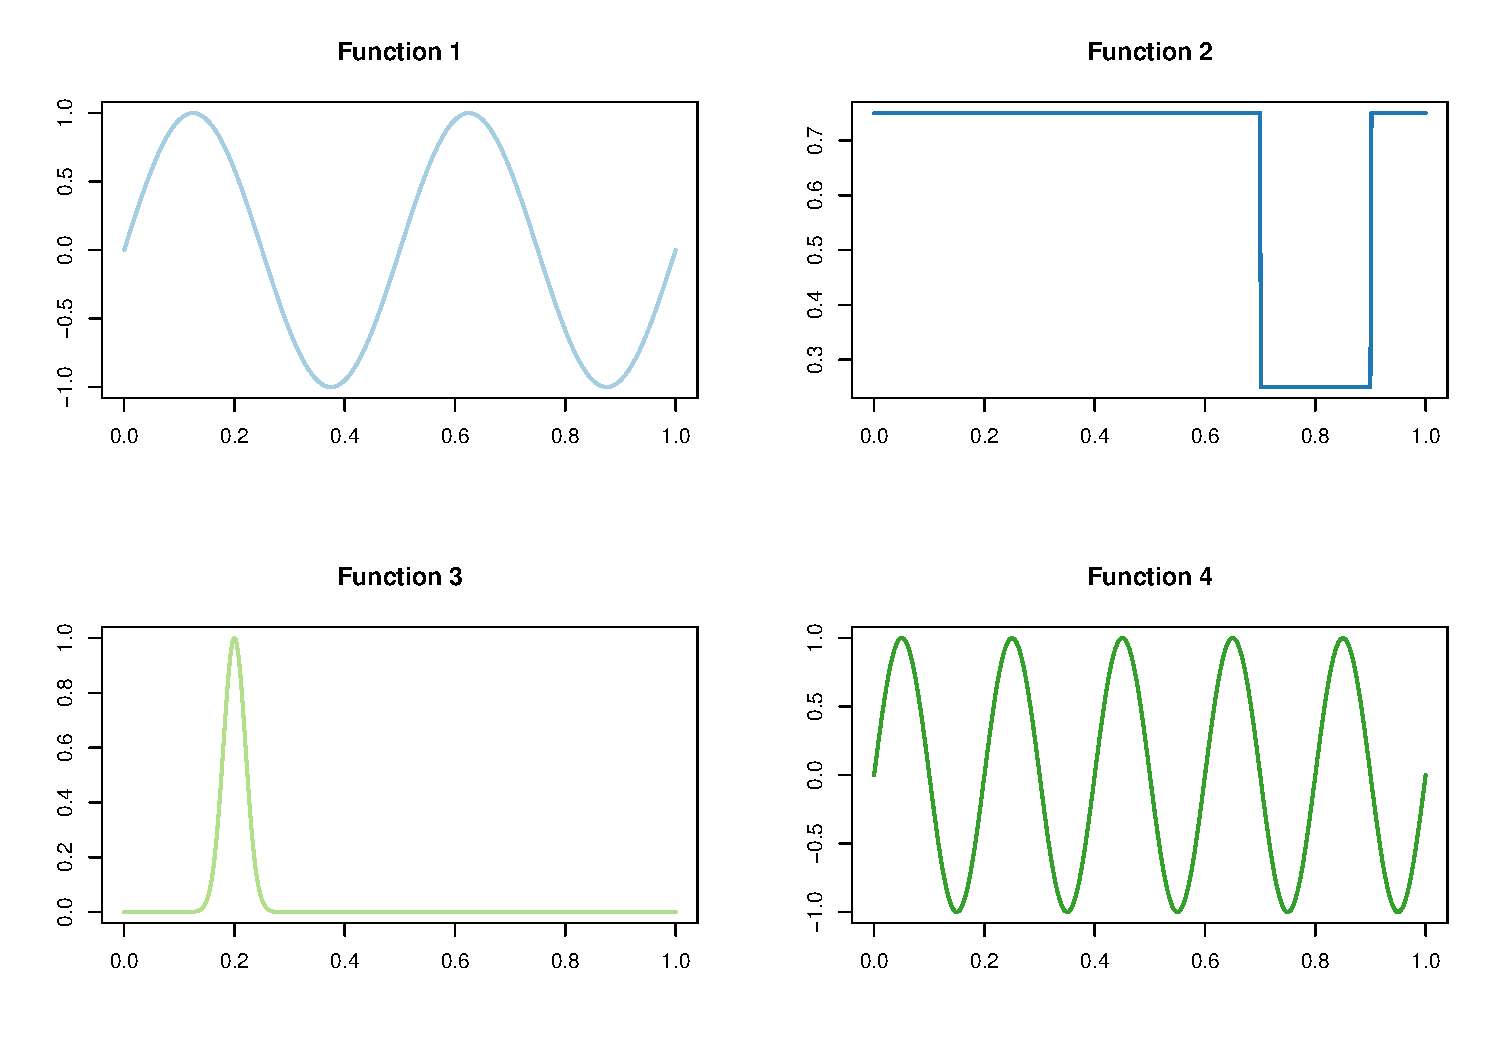
\includegraphics[width=0.5\columnwidth]{images/Fig-Simu-functions}
\par\end{centering}
\item all curves are sampled as follows:
\begin{eqnarray*}
x_{ij}(t)|Z_{ik}W_{jl}=1\sim\mathcal{N}(\mu_{kl}(t),\sigma^{2}),
\end{eqnarray*}
{\small where $\sigma=0.3$, $\mu_{11}=\mu_{21}=\mu_{33}=\mu_{42}=f_{1}$,
$\mu_{12}=\mu_{22}=\mu_{31}=f_{2}$, $\mu_{13}=\mu_{32}=f_{3}$ and
$\mu_{23}=\mu_{41}=\mu_{43}=f_{4}$.}
\item noise is added by adding $\tau\%$ of curves from other blocks.
\end{itemize}
\end{frame}


\begin{frame}{3 scenarios of simulation}
\begin{table}
\caption{\label{tab:Parameter-values}Parameter values for the three simulation
scenarios.}
\begin{small}
\begin{tabular}{|l|c|c|c|}
\hline 
Scenario & A & B & C\tabularnewline
\hline 
\hline 
$n$ (nb. of rows) & \multicolumn{3}{c|}{100}\tabularnewline
\hline 
$p$ (nb. of columns) & \multicolumn{3}{c|}{100}\tabularnewline
\hline 
$T$ (length of curves) & \multicolumn{3}{c|}{30}\tabularnewline
\hline 
$K$ (row groups nb.) & 3 & 4 & 4\tabularnewline
\hline 
$L$ (col. groups nb.) & 3 & 3 & 3\tabularnewline
\hline 
$\alpha$ (row group prop.) & $(0.333,...,0.333)$ & $(0.2,0.4,0.1,0.3)$ & $(0.2,0.4,0.1,0.3)$\tabularnewline
\hline 
$\beta$ (col. group prop.) & $(0.333,...,0.333)$ & $(0.4,0.3,0.3$) & $(0.4,0.3,0.3$)\tabularnewline
\hline 
$\tau$ (simulation noise) & 0 & 0.1 & 0.3\tabularnewline
\hline 
\end{tabular}
\end{small}
\end{table}
\end{frame}


\begin{frame}{ICL performance for choosing $(K,L)$}
\begin{table}
\begin{tabular}{|c|c|c|c|c|c|c|}
\hline 
\multicolumn{7}{|c|}{Scenario A ($K=3$, $L=3$)}\tabularnewline
\hline 
$K$\textbackslash{}$L$ & 1 & 2 & 3 & 4 & 5 & 6\tabularnewline
\hline 
1 & 0 & 0 & 0 & 0 & 0 & 0\tabularnewline
\hline 
2 & 0 & 0 & 0 & 0 & 0 & 0\tabularnewline
\hline 
3 & 0 & 0 & \textbf{100} & 0 & 0 & 0\tabularnewline
\hline 
4 & 0 & 0 & 0 & 0 & 0 & 0\tabularnewline
\hline 
5 & 0 & 0 & 0 & 0 & 0 & 0\tabularnewline
\hline 
6 & 0 & 0 & 0 & 0 & 0 & 0\tabularnewline
\hline 
\end{tabular}
\begin{tabular}{|c|c|c|c|c|c|c|}
\hline 
\multicolumn{7}{|c|}{Scenario B ($K=4$, $L=3$)}\tabularnewline
\hline 
$K$\textbackslash{}$L$ & 1 & 2 & 3 & 4 & 5 & 6\tabularnewline
\hline 
1 & 0 & 0 & 0 & 0 & 0 & 0\tabularnewline
\hline 
2 & 0 & 0 & 0 & 0 & 0 & 0\tabularnewline
\hline 
3 & 0 & 0 & 0 & 0 & 0 & 0\tabularnewline
\hline 
4 & 0 & 0 & \textbf{70} & 0 & 1 & 0\tabularnewline
\hline 
5 & 0 & 0 & 26 & 1 & 0 & 0\tabularnewline
\hline 
6 & 0 & 0 & 2 & 0 & 0 & 0\tabularnewline
\hline 
\end{tabular}
\begin{tabular}{|c|c|c|c|c|c|c|}
\hline 
\multicolumn{7}{|c|}{Scenario C ($K=4$, $L=3$)}\tabularnewline
\hline 
$K$\textbackslash{}$Q$ & 1 & 2 & 3 & 4 & 5 & 6\tabularnewline
\hline 
1 & 0 & 0 & 0 & 0 & 0 & 0\tabularnewline
\hline 
2 & 0 & 0 & 17 & 0 & 0 & 0\tabularnewline
\hline 
3 & 0 & 0 & \textbf{77} & 0 & 0 & 0\tabularnewline
\hline 
4 & 0 & 0 & 5 & 0 & 0 & 0\tabularnewline
\hline 
5 & 0 & 0 & 1 & 0 & 0 & 0\tabularnewline
\hline 
6 & 0 & 0 & 0 & 0 & 0 & 0\tabularnewline
\hline
\end{tabular}
\end{table}
\end{frame}

\begin{frame}{Co-clustering results for scenario B}
\begin{figure}
\begin{centering}
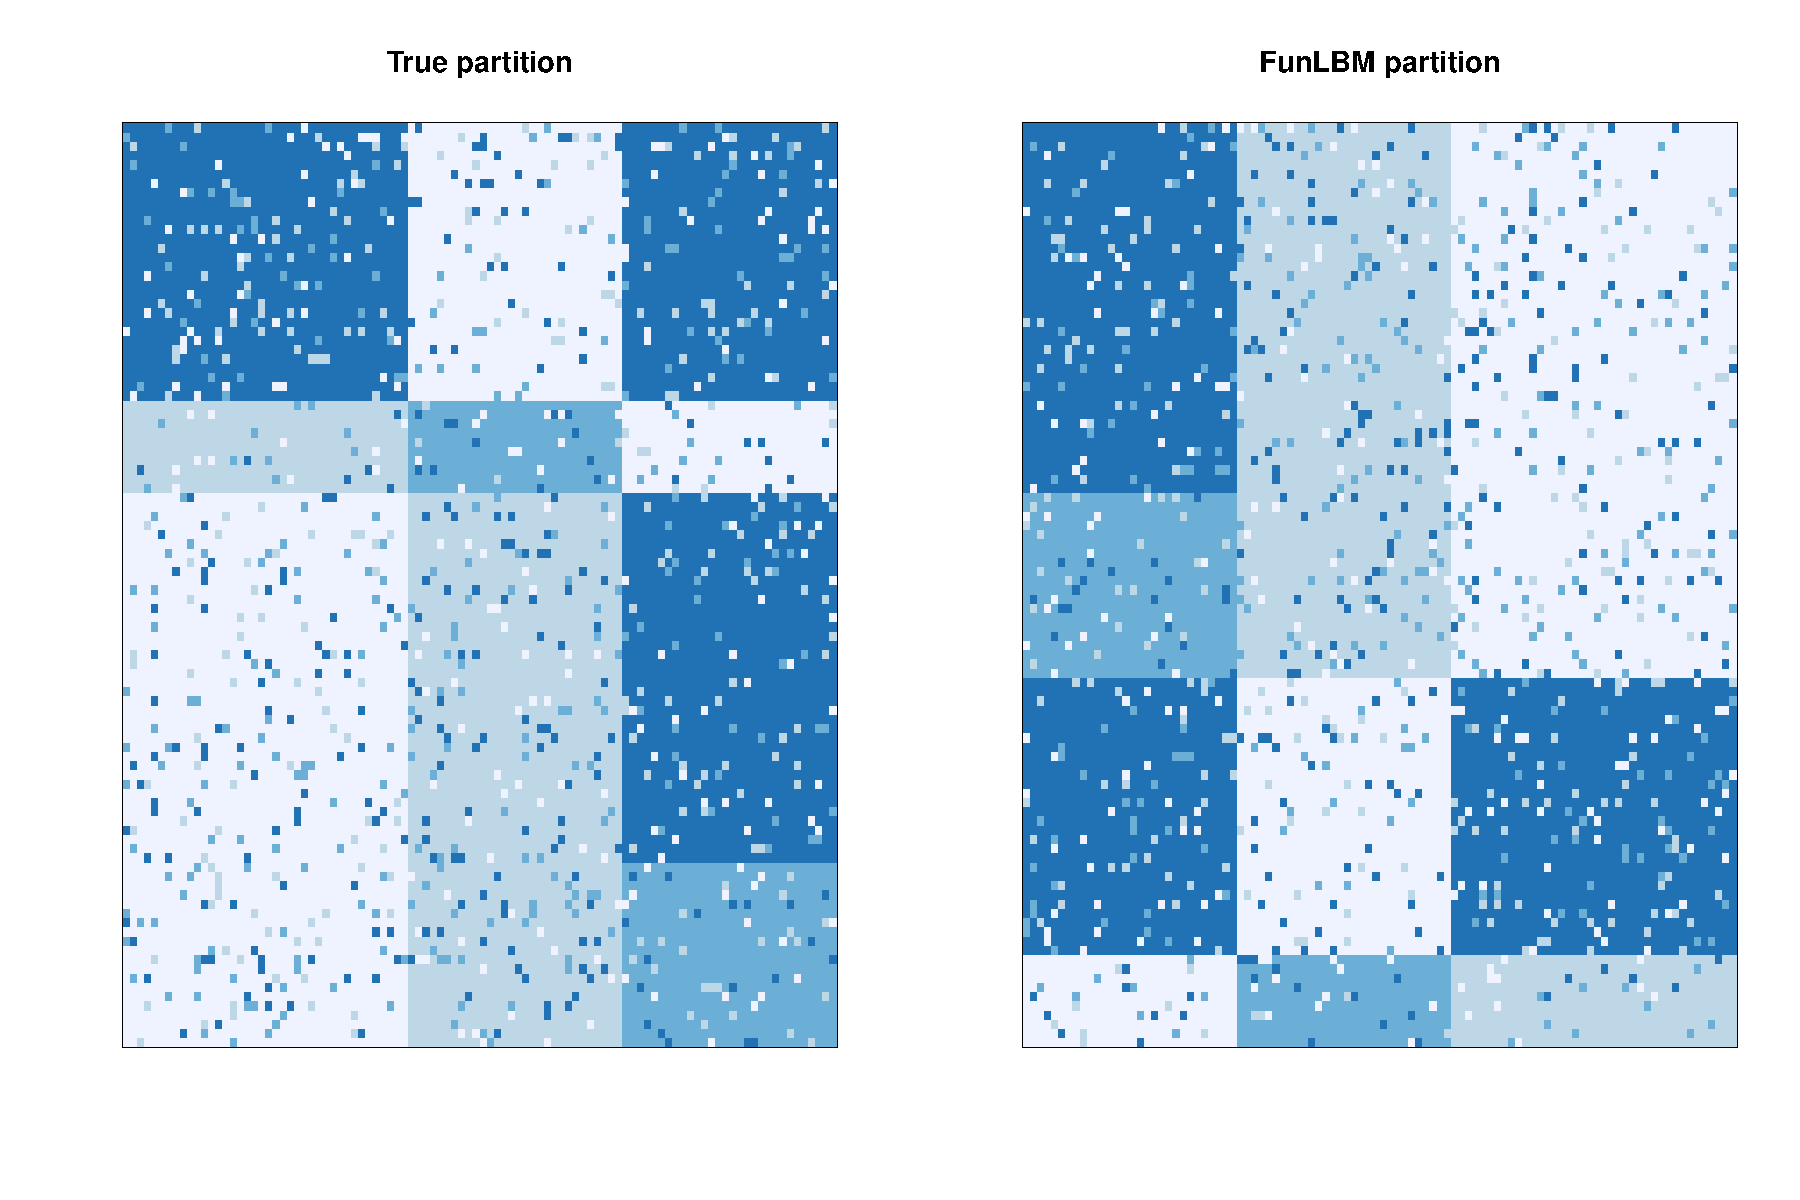
\includegraphics[width=0.9\columnwidth]{images/Fig-Simu-clustering2}
\par\end{centering}
\end{figure}
\end{frame}

\begin{frame}{Co-clustering results}
\begin{figure}
\begin{centering}
\begin{tabular}{c}
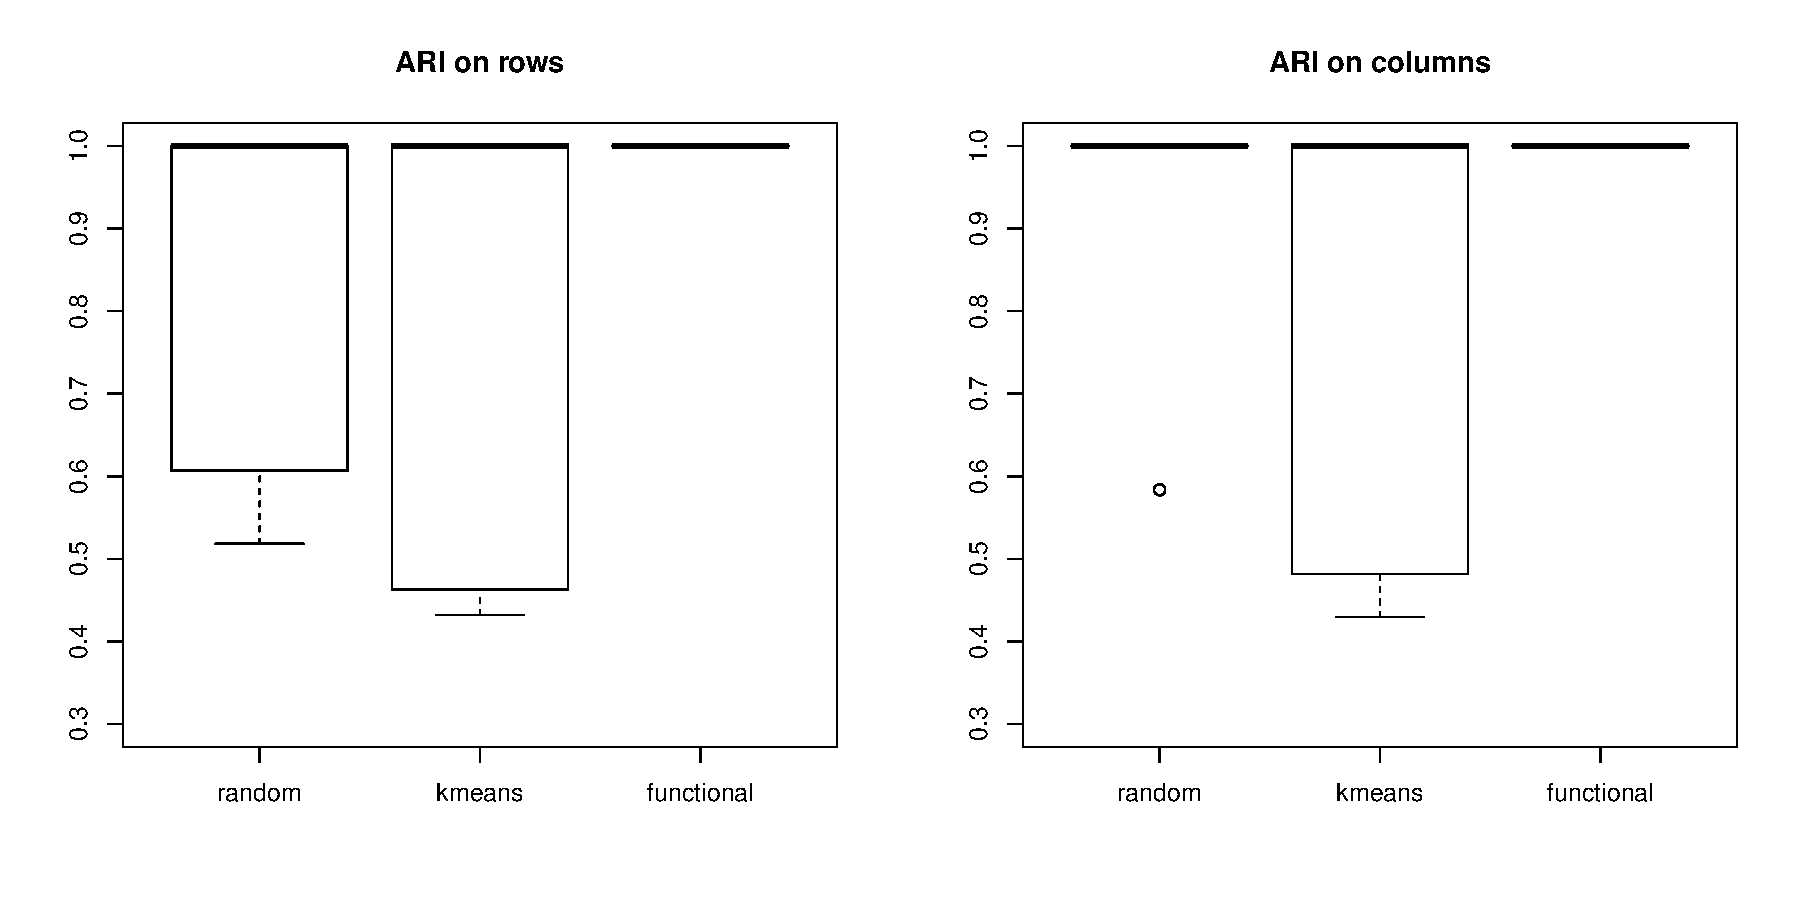
\includegraphics[width=0.5\columnwidth]{images/simu-init-A}
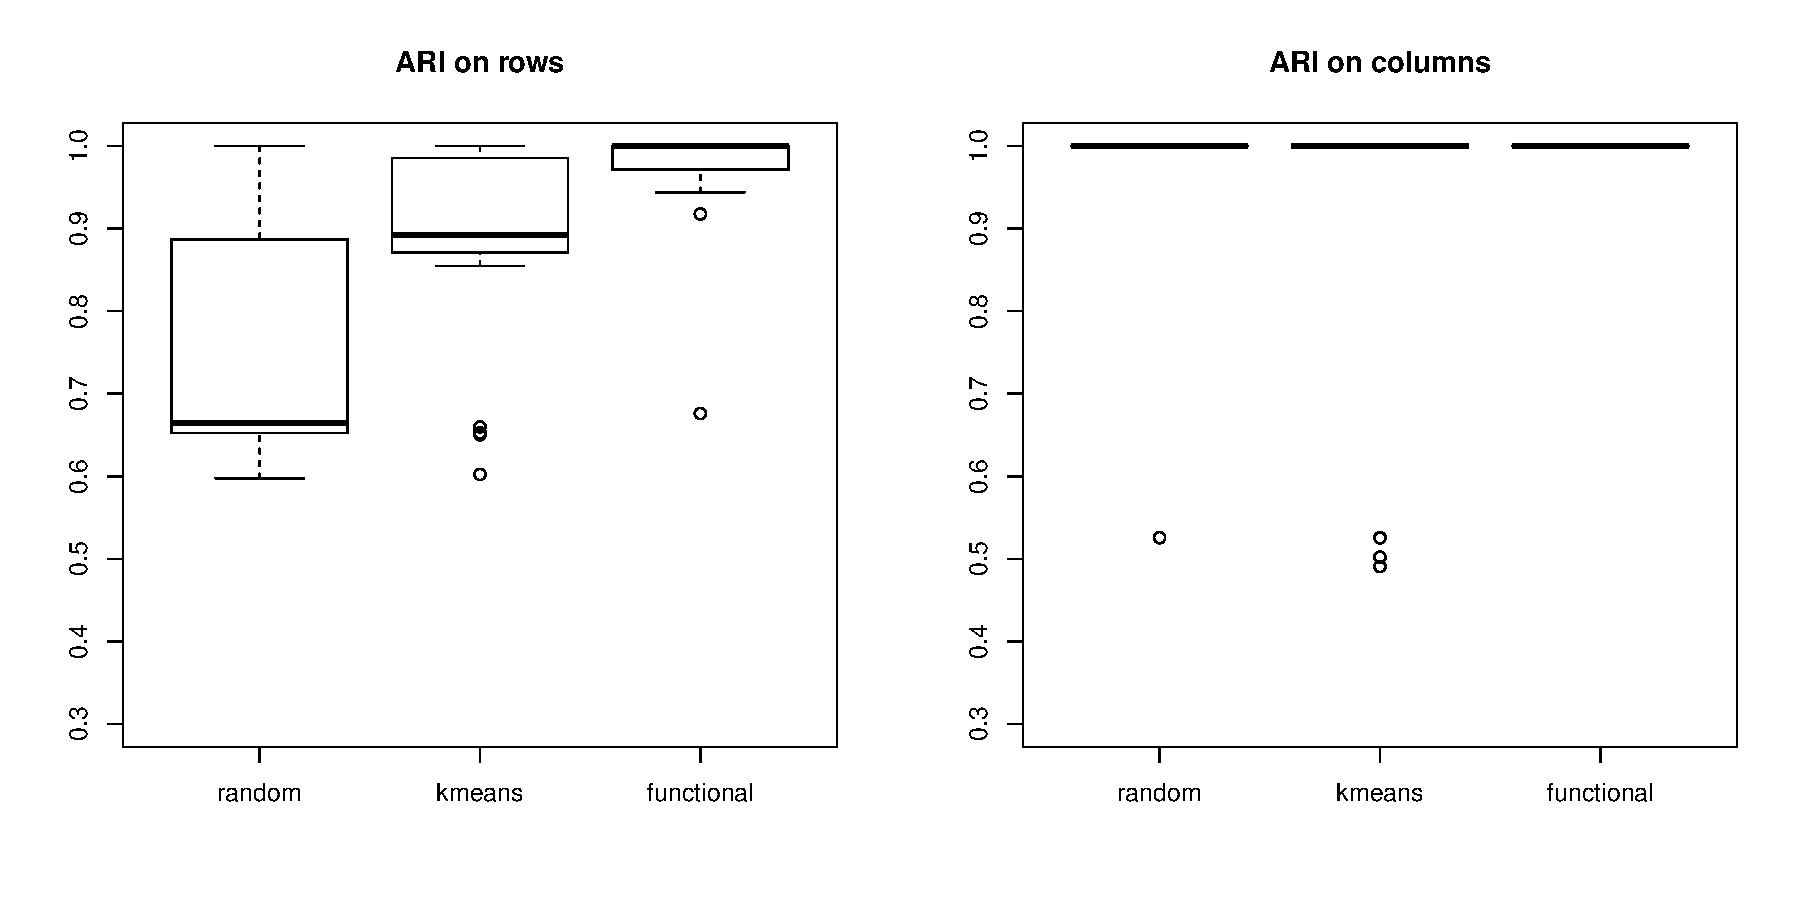
\includegraphics[width=0.5\columnwidth]{images/simu-init-B}\tabularnewline
(a) scenario A \hspace{4cm}(b) scenario B
\tabularnewline
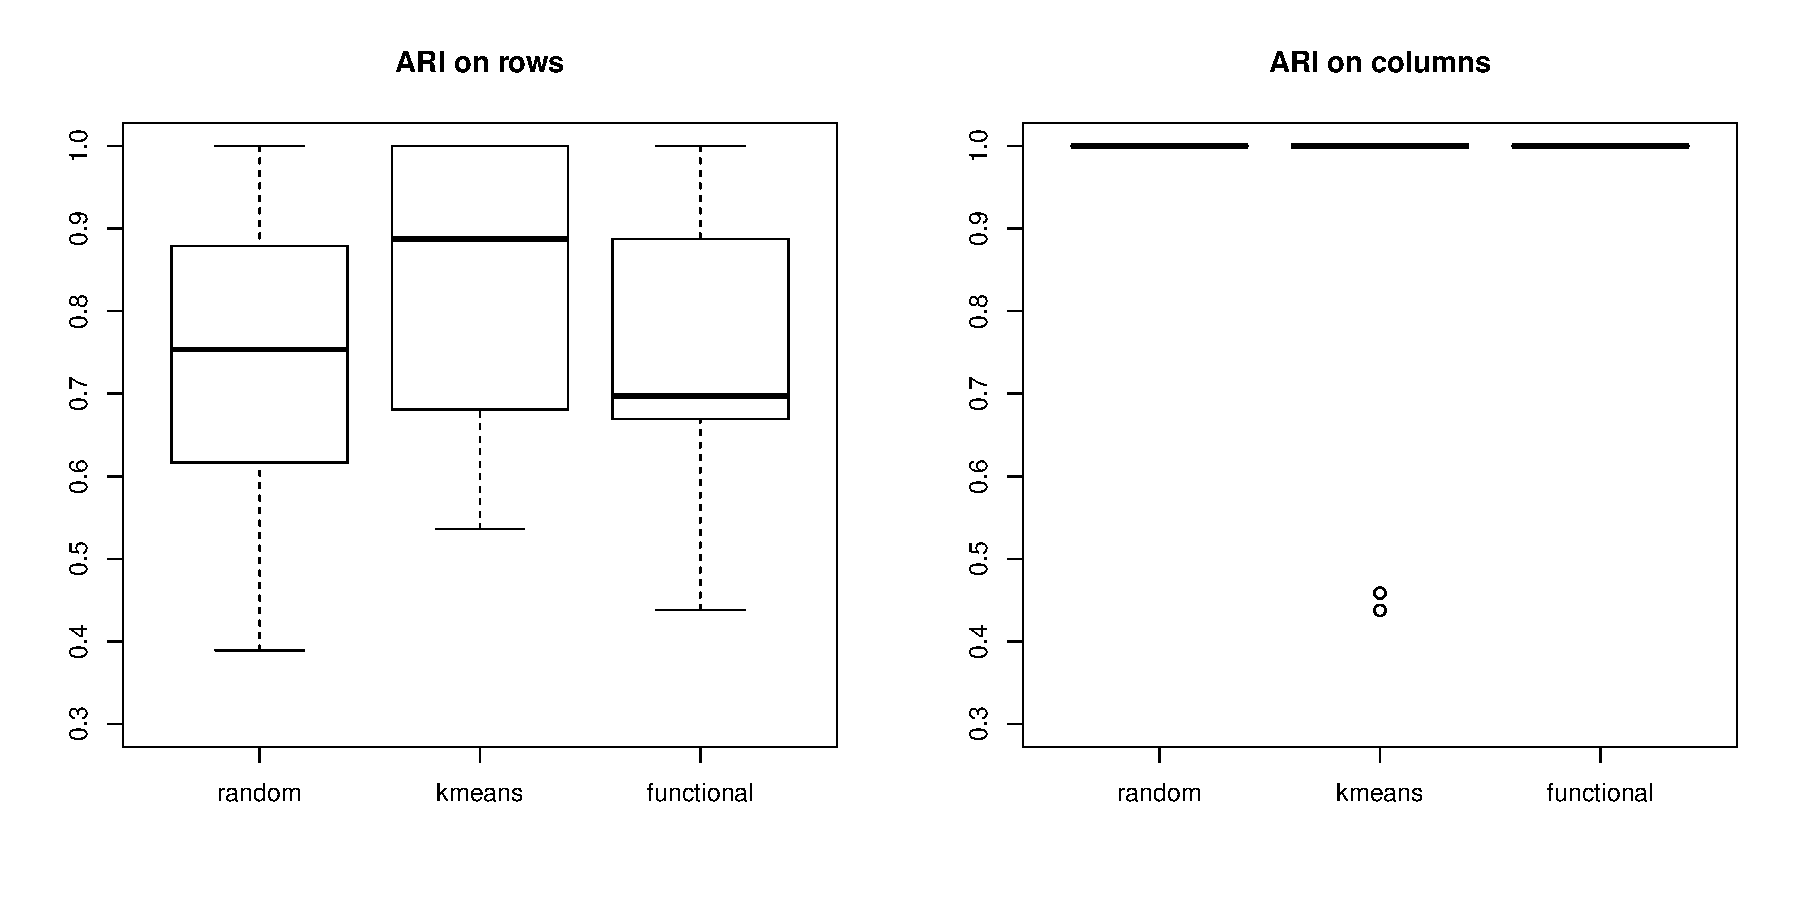
\includegraphics[width=0.5\columnwidth]{images/simu-init-C}\tabularnewline
(c) scenario C\tabularnewline
\end{tabular}
\par\end{centering}
\caption{\label{fig:simu-init}Adjusted Rand index values for the different
initialization procedures on the three simulation scenarios.}
\end{figure}
\end{frame}

\section{Application on EDF consumption curves}


\begin{frame}
\frametitle{The data \hspace{7cm} 
\includegraphics[height=.7cm,angle=0]{images/EDF.jpg}}
\begin{itemize}
\item \relief{electricity consumption} measured by Linky meters for EDF
\item \relief{27 millions} of customers / \relief{730 daily} consumption over 2 years
\begin{figure}
%\begin{center}
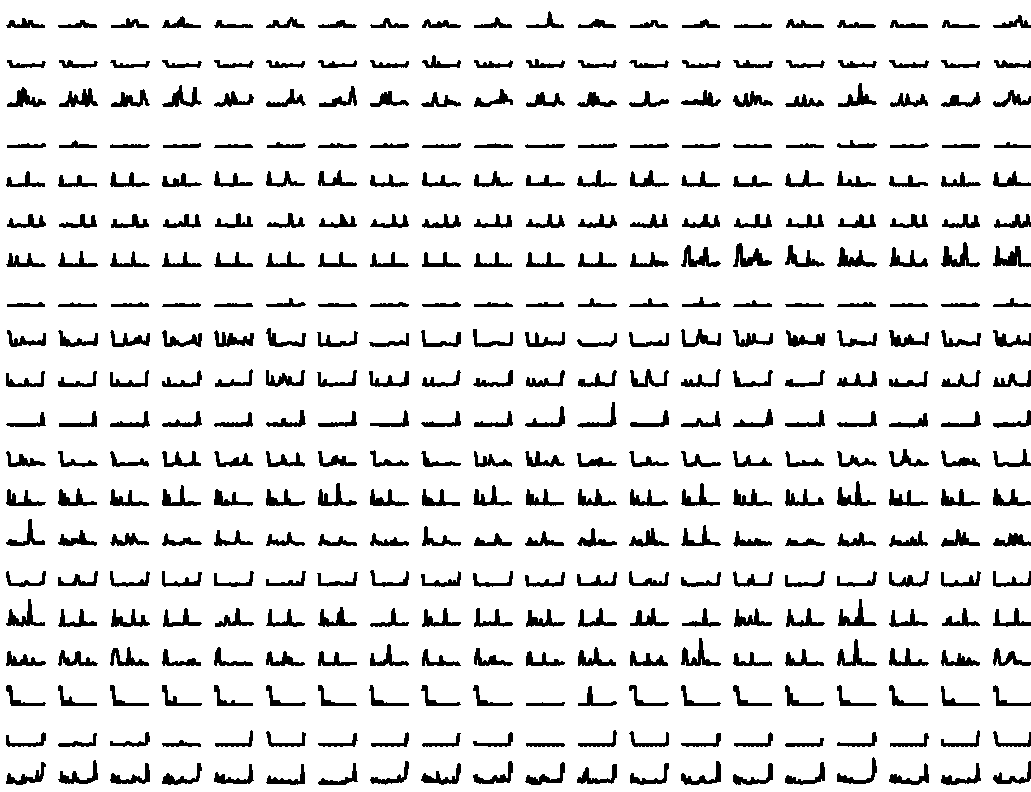
\includegraphics[width=6cm]{images/dataEDF.pdf}
%\end{center}
\caption{Sample of 20 consumptions for 20 days}
\end{figure}
\end{itemize}
\end{frame}

\begin{frame}{ICL values (choice of $(K,L)$)}
\begin{figure}
\begin{centering}
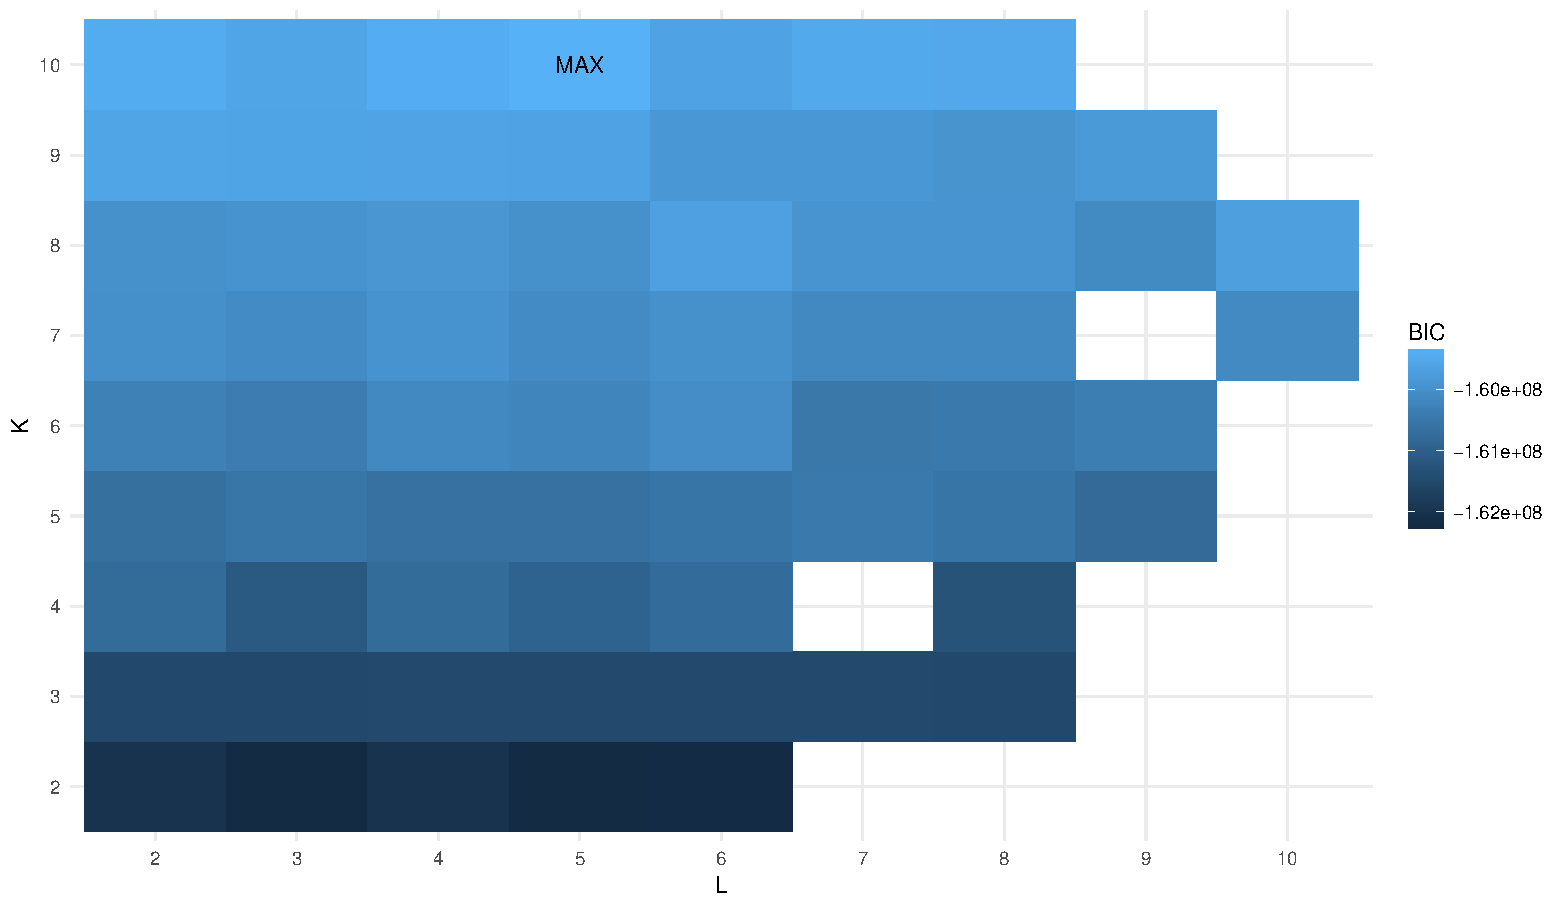
\includegraphics[width=0.9\columnwidth]{images/graph-bic-heatmap.pdf}
\par\end{centering}
\end{figure}
\end{frame}

\begin{frame}{Clustering of columns (dates)}
\begin{figure}
\begin{centering}
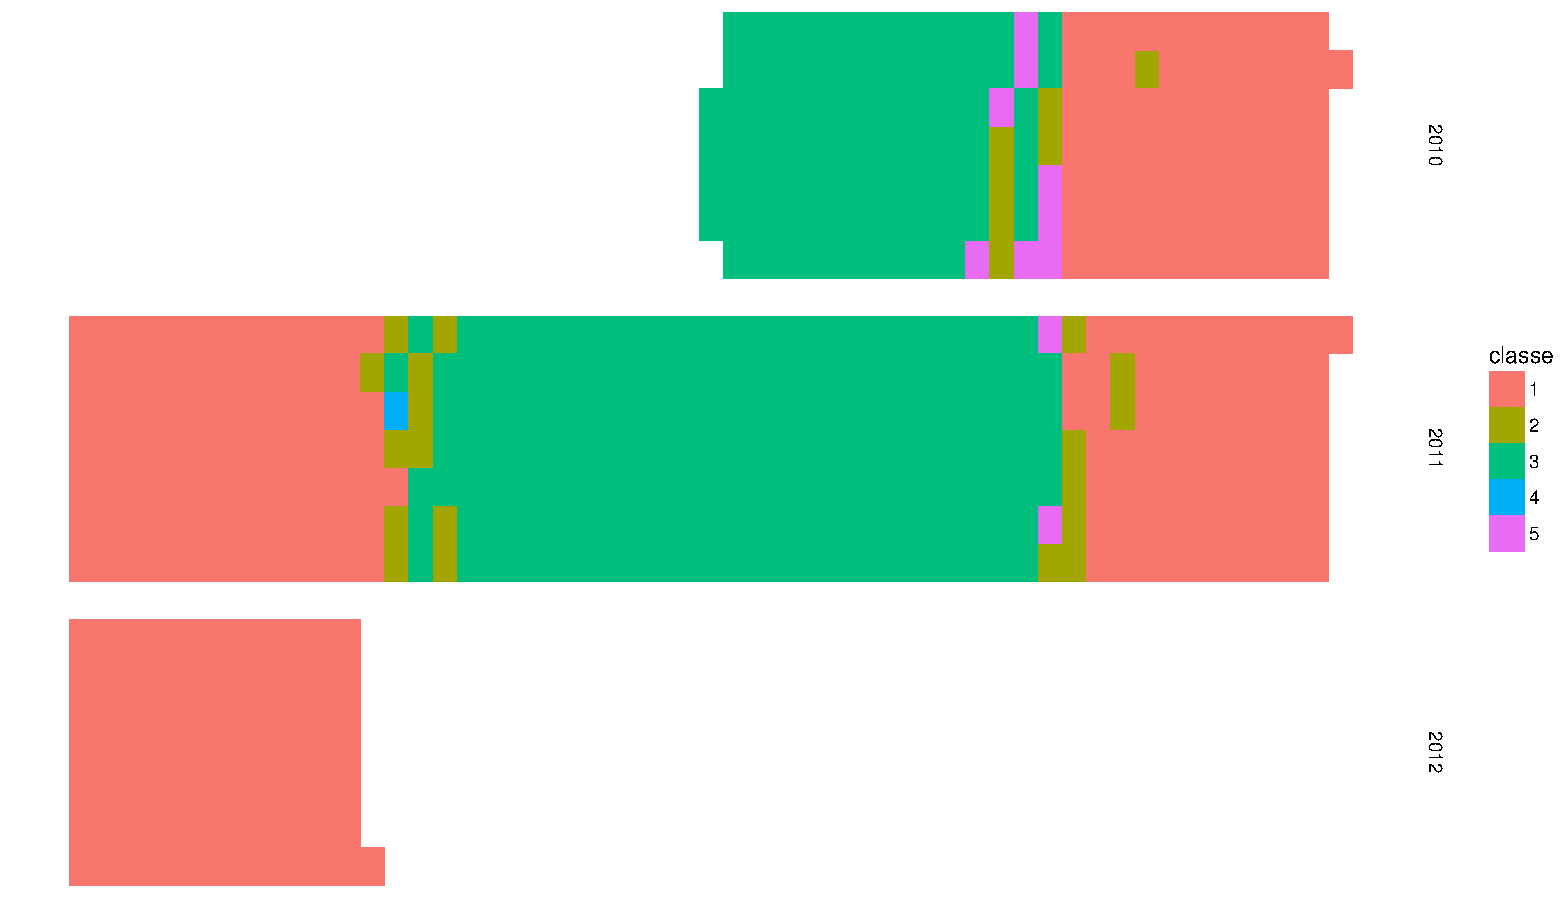
\includegraphics[width=0.9\columnwidth]{images/graph-dates.pdf}
\par\end{centering}
\end{figure}
\end{frame}

\begin{frame}{Average consumption curves of each block}
\begin{figure}
\begin{centering}
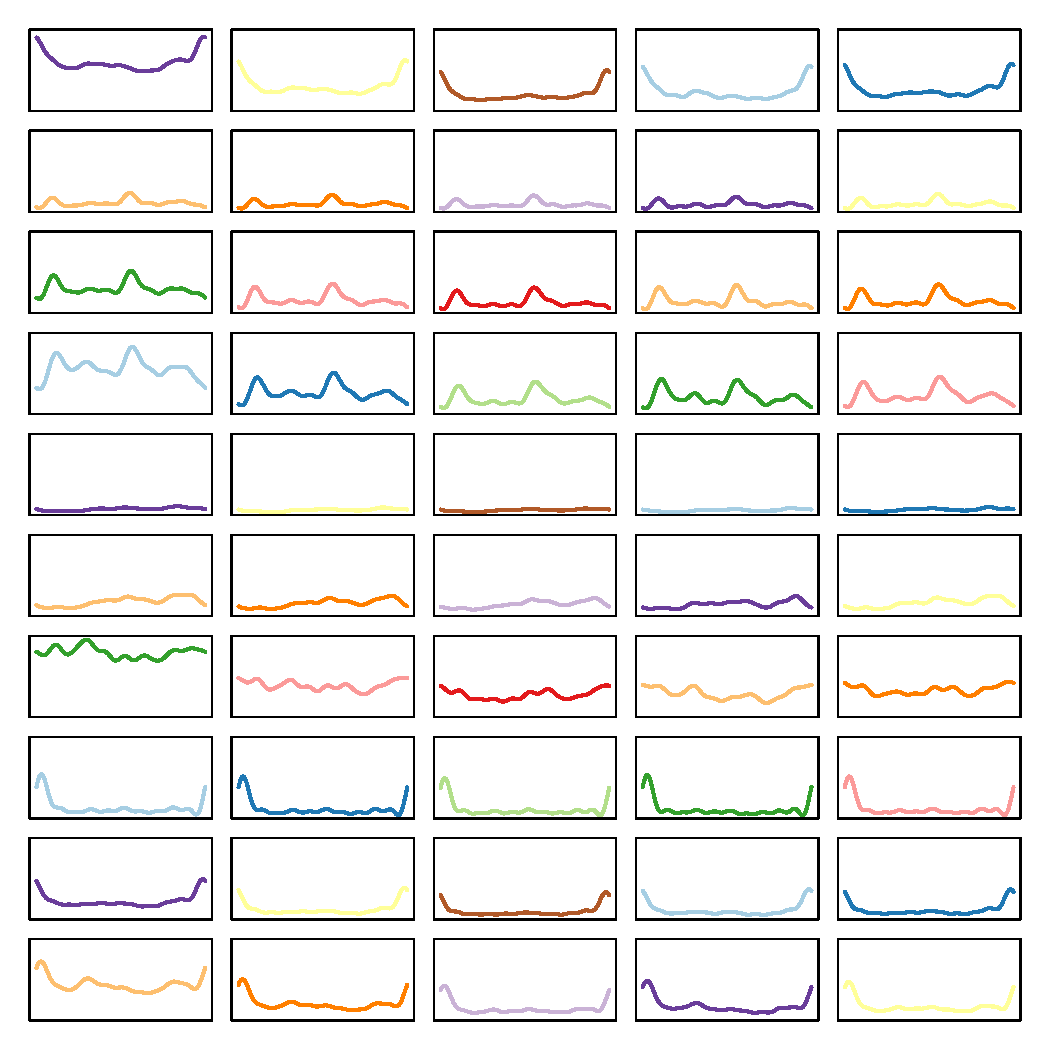
\includegraphics[width=0.9\columnwidth,height=7cm]{images/graph-adjacency.pdf}
\par\end{centering}
\end{figure}
\end{frame}

\begin{frame}{Geographical clusters distributions}
\begin{figure}
\begin{centering}
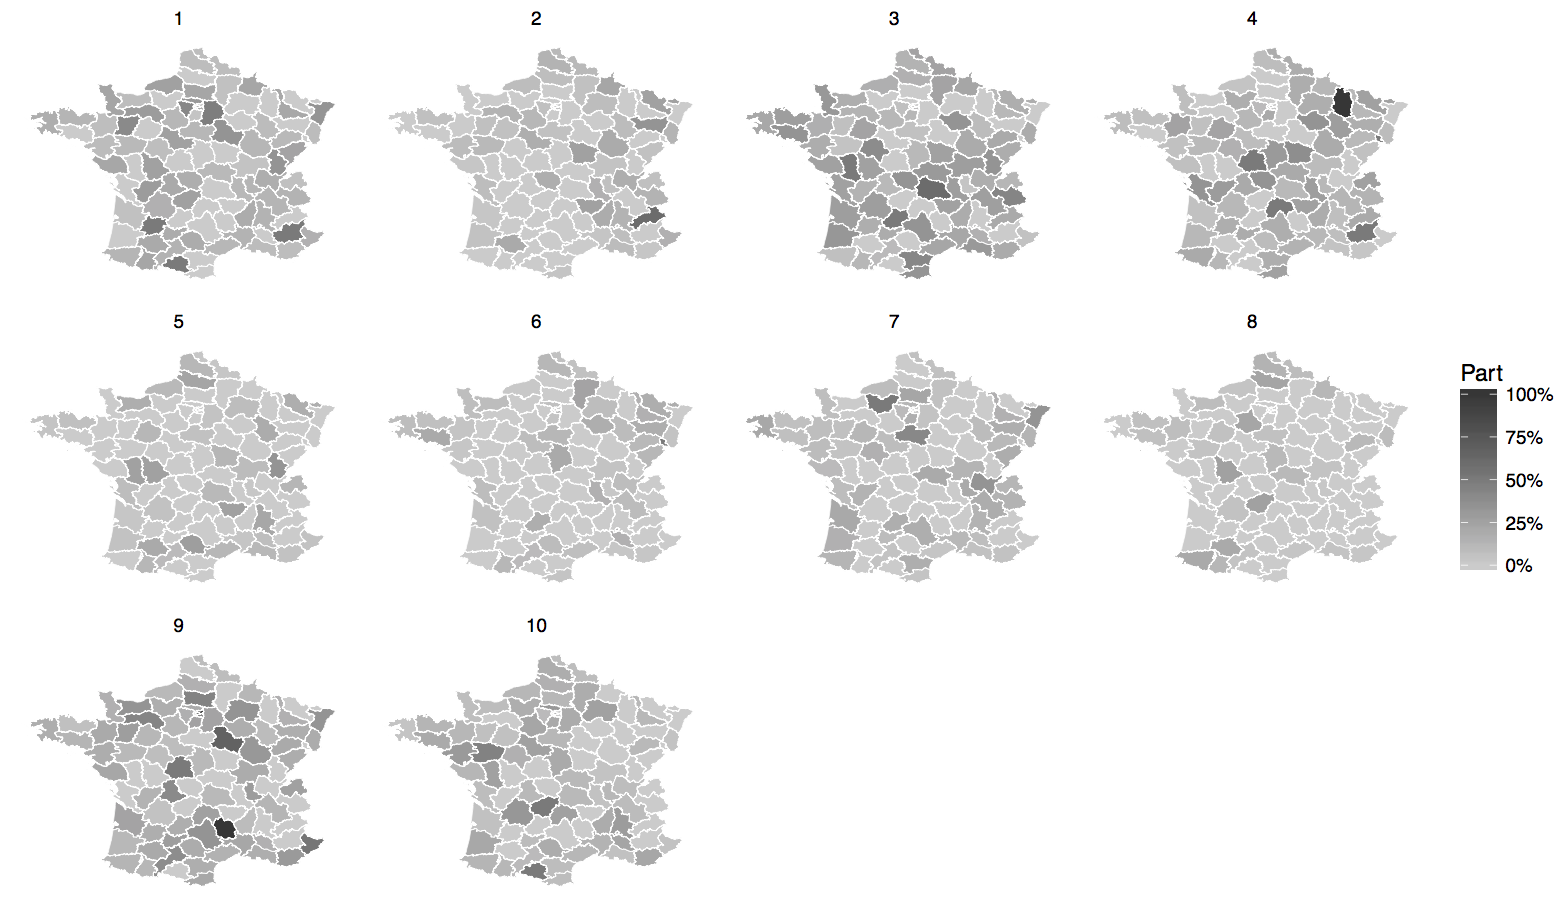
\includegraphics[width=0.9\columnwidth]{images/graph-cartes.png}
\par\end{centering}
\caption{Proportions on households per French departments in each of the 10 clusters found by FunLBM.}
\label{fig:EDF-ICL}
\end{figure}
\end{frame}

\begin{frame}{Conclusions}
\begin{block}{Results}
\begin{itemize}
\item \relief{real data} application needs development of a \relief{co-clustering algorithm for functional data}
\item co-clustering algorithm has been developed based on a \relief{functional Latent Block model}
\item numerical experiments show the \relief{efficiency of SEM-Gibbs} for model estimation as well as \relief{ICL-BIC}  for selecting of the number of blocks
\item Results on EDF data are significant
\end{itemize}
\end{block}
\begin{block}{References}
\begin{itemize}
\item Bouveyron, C. and Jacques, J. (2011), Model-based Clustering of Time Series in Group-specific Functional Subspaces, Advances in Data Analysis and Classification, 5[4], 281-300.
\item  Govaert, G. and Nadif, M. (2013). Co-Clustering. Wiley-ISTE.
\end{itemize}
\end{block}
\end{frame}

\begin{frame}[fragile]{R Package}
\begin{block}{funLBM}
\begin{itemize}
	\item Available on CRAN : \url{https://cran.r-project.org/package=funLBM}
\end{itemize}
\end{block}
\begin{block}{Example}
\lstset{language=R}
\begin{lstlisting}
library(funLBM)
data(Velib)
# Co-clustering
out = funLBM(Velib$data, K = 4, L = 2)
# Visualization of results
plot(out, type = 'blocks')
plot(out, type = 'proportions')
plot(out, type = 'means')
\end{lstlisting}
\end{block}
\end{frame}

\end{document}